\scanpage{32}
that $\underline{\operatorname{Hom}}_S(X,Y)$ is representable (\unsure{aby|any} $Y$ locally of finite presentation \inserted{and separated} over $k$); if we do not make any assumption on $X$ except properness over $k$, the previous assumption becomes true after finite ground-field extension $k'/k$, so that we get that for every $Y$ as above, $\underline{\operatorname{Hom}}_S(X,Y)\times_S\operatorname{Spec}(k')$ is representable. From this \unsure{Matsumurds|Matsumura's} theorem stated at the beginning follows in a standart way by \unsure{descebt|descent} arguments. The result holds too for $\underline{\operatorname{Isom}}_k(X,Y)$ instead of $\underline{\operatorname{Aut}}_k(X)$, but as you probably know, $\underline{\operatorname{Hom}}_S(X,Y)$ is not always representable, even if $X$ is a quadratic extension of $S=\operatorname{Spec}k$, $Y$ being proper non projective.

Over an arbitrary base $S$, one can give a fairly general statement of a representability theorem, the points radicial over $k$ used above being replaced by suitable flat subschemes of $X$. As \deleted{applications} \inserted{particular cases}, we get for instance that if $X$ has integral \unsure{geométric|geometric} fibers and a \unsure{sectionx|section} \inserted{along which $X$ is smooth,} then $\underline{\operatorname{Hom}}_S(X,Y)$ is representable; and if $X$ has \figure{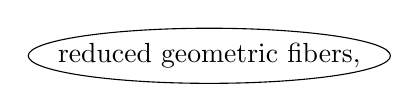
\begin{tikzpicture}[baseline=(m.base)]\node[inner sep=2pt] (m) at (0,0) {reduced geometric fibers,};\draw (0,0) ellipse[x radius=2.3cm,y radius=0.35cm];\end{tikzpicture}} then $\underline{\operatorname{Hom}}_S(X,Y)$ is representable locally for the étale topology over $S$. Also, if $Y$ is quasi-projective over $S=\operatorname{Spec}k$, then $\underline{\operatorname{Hom}}_S(X,Y)$ is representable.

To \unsure{gix|fix} the ideas, I gave the statements for $\underline{\operatorname{Hom}}_S(X,Y)$, but one has quite analogous resultst of course for the $\prod_{X/S}P/X$ fonctors, which I guess will imply rather formally the other \unsure{onesx|ones}.

If you are interested, I can send you a photocopy of the statement of the general theorem of representability I alluded to\unsure{,} above, and a couple of corollaries (I already listed here the most striking ones).

Sincerely your's
% archive foliation: 31
